\section{Архитектура прототипа}
\label{sec:development}

Разработанное программное обеспечение предстваляет из себя библиотеку кода,
написанную на языке \csharp{}. Библиотека предназначена для демонстрирования
использования нейронных сетей для сжатия графической информации.

Одним из важных решений, которое было принято в начале проектирования модуля работы
с нейронными сетями, было разделение реализации от абстрактной модели. Это решение
позволило сначало реализовать сам алгоритм без реализации его компонентов. Так же это позволило в дальнейшем протестировать составные части.

В ходе разработки активно использовались паттерны Стратегия, Абстрактная Фабрика, Строитель.
Стратегия --- поведенческий шаблон проектирования, предназначенный для определения семейства алгоритмов,
инкапсуляции каждого из них и обеспечения их взаимозаменяемости. Это позволяет выбирать алгоритм путем
определения соответствующего класса. Шаблон позволяет менять выбранный алгоритм независимо от объектов-клиентов, которые его используют~\cite{development_patterns}.

Абстрактная фабрика --- порождающий шаблон проектирования, позволяющий изменять поведение системы,
варьируя создаваемыми объектами, при этом сохраняя интерфейсы. Он позволяет создавать целые группы
взаимосвязанных объектов, которые, будучи созданными одной фабрикой, реализуют общее поведение.
Шаблон реализуется созданием абстрактного класса Factory, который представляет собой интерфейс для
создания компонентов системы. Затем пишутся классы, реализующие этот интерфейс~\cite{development_patterns}.

Строитель --- отделяет конструирование сложного объекта от его представления,
так что в результате одного и того же процесса конструирования могут получаться разные представления~\cite{development_patterns}.

На рисунке~\ref{fig:modules} представлена схема модулей системы.
В данной секции будет приведено описение секции Interfaces. В ней содержится абстрактное представление
системы.

\begin{figure}[ht]
\centering
  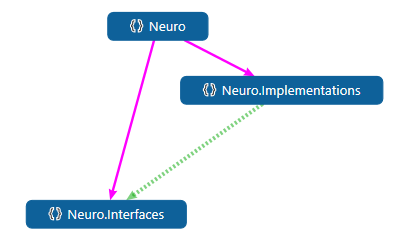
\includegraphics[scale=1]{modules.png}
  \caption{ Схема модулей программы }
  \label{fig:modules}
\end{figure}

\begin{figure}[ht]
\centering
  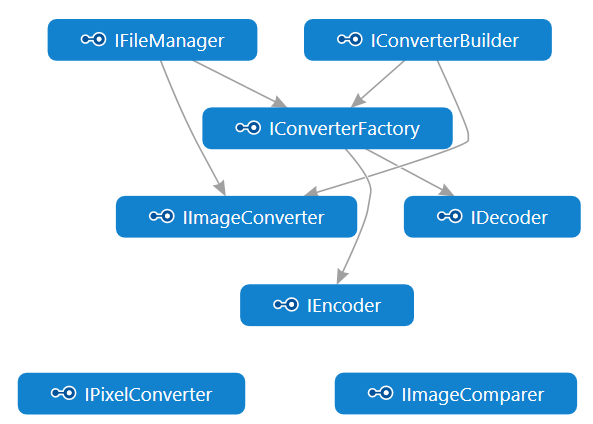
\includegraphics[scale=0.6]{interfaces.png}
  \caption{ Схема интерфейсов программы }
  \label{fig:interfaces}
\end{figure}
В системе присутствует 8 интерфейсов(рисунок~\ref{fig:interfaces}):
\begin{itemize}
  \item IPixelConverter --- преобразователь одного пикселя в сигнал;
  \item IImageConverter --- преобразователь матрицы пикселей в матрицу сигналов;
  \item IEncoder --- интерфейс объекта кодирования сигналов;
  \item IDecoder --- интерфейс объекта декодирования сигналов;
  \item IConverterFactory --- интерфейс фабрики, которая возвращает пару кодер/декодер;
  \item IConverterBuilder --- интерфейс строителя, который по исходным данным создает фабрику кодеров/декодеров;
  \item IFileManager --- интерфейс для загрузки/сохранения исходных и сжатых изображений;
  \item IImageComparer --- интекфейс для алгоритмов оценки качества полученных изображений.
\end{itemize}

\subsubsection{Интерфейс IPixelConverter}
\label{subsub:development:types:ipixelconverter}

\begin{figure}[ht]
\centering
  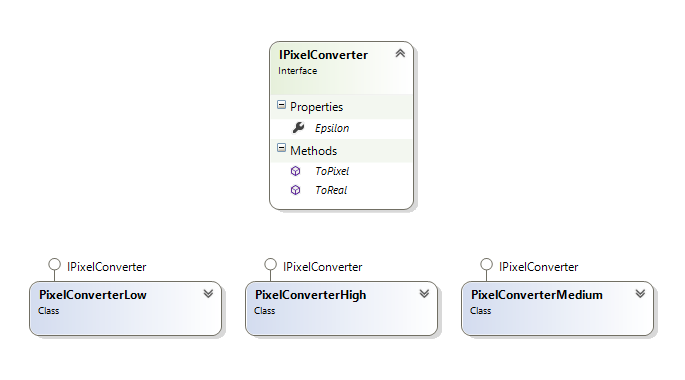
\includegraphics[scale=0.6]{IPixelConverter.png}
  \caption{ Интерфейс IPixelConveter }
  \label{fig:ipixelconverter}
\end{figure}
IPixelConverter --- представляет интерфейс для конвертации сигналов в пиксели и наоборот(рисунок~\ref{fig:ipixelconverter}).

В нем представлены методы:
\begin{itemize}
  \item ToPixel() --- конвертация сигнала в пиксель;
  \item ToReal() --- конфертация пикселя в сигнал.
\end{itemize}

В прототипе представлены 3 реализации:
\begin{itemize}
  \item PixelConverterLow --- преобразует 256-цветовой пиксель с глубиной дискретизации 8;
  \item PixelConverterMedium --- преобразует 256-цветовой пиксель с глубиной дискретизации 32;
  \item PixelConverterHigh --- преобразует 256-цветовой пиксель с глубиной дискретизации 256.
\end{itemize}

\subsubsection{Интерфейс IImageConverter}
\label{subsub:development:types:iimageconverter}

\begin{figure}[ht]
\centering
  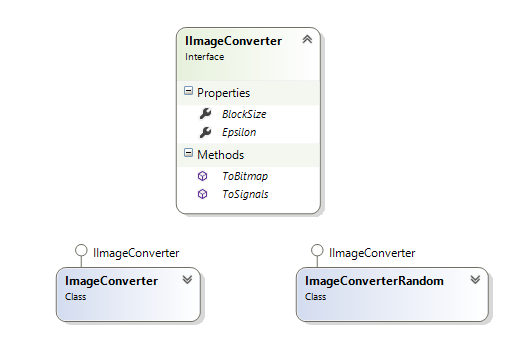
\includegraphics[scale=0.6]{IImageConverter.png}
  \caption{ Интерфейс IImageConverter }
  \label{fig:iimageconverter}
\end{figure}
IImageConverter --- представляет интерфейс для преобразования матрицы пикселей в матрицу сигналов и
преобразования матрицы сигналов в матрицу пикселей, при помощи указанного перобразвателя который наследует интерфейс IPixelConverter(рисунок~\ref{fig:iimageconverter}).

В нем представлены методы и свойства:
\begin{itemize}
  \item BlockSize --- размер стороны блока;
  \item Epsilon --- шаг дискретизации;
  \item ToBitmap() --- метод преобразования матрицы сигналов в матрицу пикселей;
  \item ToSignals() --- метод преобразования матрицы пикселей в матрицу сигналов.
\end{itemize}

В прототипе представлены 3 реализации:
\begin{itemize}
  \item ImageConverter --- преобразует матрицу пикселей в матрицу сигналов соответвующего размера;
  \item ImageConverterRandom --- преобразует матрицу пикселей в матрицу сигналов и выделяет только необходимое
  количество блоков для использования в алгоритме обучения нейронной сети.
\end{itemize}

\subsubsection{Интерфейс IEncoder}
\label{subsub:development:types:iencoder}

\begin{figure}[ht]
\centering
  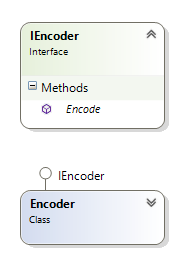
\includegraphics[scale=0.6]{IEncoder.png}
  \caption{ Интерфейс IEncoder }
  \label{fig:iencoder}
\end{figure}
IEncoder --- представляет интерфейс для преобразования матрицы сигналов в матрицу сигналов меньшей размерности (рисунок~\ref{fig:iencoder}).

В нем представлены методы:
\begin{itemize}
  \item Encode() --- метод преобразования матрицы сигналов одной размерности в матрицу сигналов другой размерности.
\end{itemize}

В прототипе представлена одна реализация Encoder, которая создается на основе полученной нейронной сети.

\subsubsection{Интерфейс IDecoder}
\label{subsub:development:types:idecoder}

\begin{figure}[ht]
\centering
  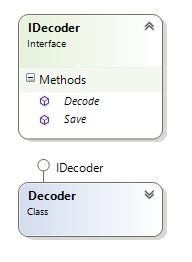
\includegraphics[scale=0.6]{IDecoder.png}
  \caption{ Интерфейс IDecoder }
  \label{fig:idecoder}
\end{figure}
IDecoder --- представляет интерфейс для преобразования матрицы сигналов малой размерности в матрицу сигналов исходной размерности (рисунок~\ref{fig:idecoder}).

В нем представлены методы:
\begin{itemize}
  \item Decode() --- метод преобразования матрицы сигналов малой размерности в матрицу сигналов исходной размерности.
  \item Save() --- метод сохраняющий объект IDecoder в Stream(класс представляющий поток данных).
\end{itemize}

В прототипе представлена одна реализация Decoder, которая создается на основе полученной нейронной сети или загружается из Stream.

\subsubsection{Интерфейс IConverterFactory}
\label{subsub:development:types:iconverterfactory}

\begin{figure}[ht]
\centering
  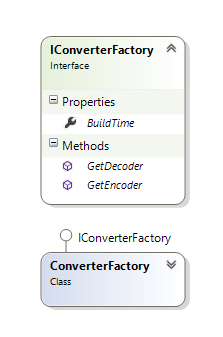
\includegraphics[scale=0.6]{IConverterFactory.png}
  \caption{ Интерфейс IConverterFactory }
  \label{fig:iconverterfactory}
\end{figure}
IConverterFactory --- представляет интерфейс, с использованием которого можно получить объекты кодера и декодера,
а также узнать время обучения нейронной сети для их создания (рисунок~\ref{fig:iconverterfactory}).

В нем представлены методы и свойства:
\begin{itemize}
  \item BuildTime --- время обучения нейронной сети;
  \item GetEncoder() --- метод, который предоставляет объект IEncoder;
  \item GetDecoder() --- метод, который предоставляет объект IDecoder.
\end{itemize}

В прототипе представлена одна реализация ConverterFactory, которая создается объектом строителя ConverterBuilder.

\subsubsection{Интерфейс IConverterBuilder}
\label{subsub:development:types:iconverterbuilder}

\begin{figure}[ht]
\centering
  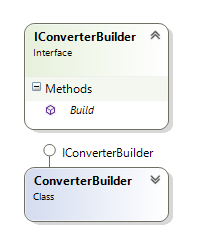
\includegraphics[scale=0.6]{IConverterBuilder.png}
  \caption{ Интерфейс IConverterBuilder }
  \label{fig:iconverterbuilder}
\end{figure}
IConverterBuilder --- представляет интерфейс, c помощью которого можно создавать объекты фабрик кодеров и декодеров.(рисунок~\ref{fig:iconverterbuilder}).
Использование паттерна строитель, позволяет манипулировать характеристиками нейронной сети, глубиной дискретизации.
Интерфейс позволяет изменять степень сжатия, что позволяет манипулировать размером конечного файла и качеством конечного изображения.

В нем представлены методы и свойства:
\begin{itemize}
  \item Build() --- метод котрый принимает на вход IImageConverter, Bitmap, размер исходного блока,
  размер выходного блока и строит фабрику кодеров/декодеров.
\end{itemize}

В прототипе представлена одна реализация ConverterBuilder, которая создает фабрику кодеров/декодеров для проведения исследования.

\subsubsection{Интерфейс IFileManager}
\label{subsub:development:types:ifilemanager}

\begin{figure}[ht]
\centering
  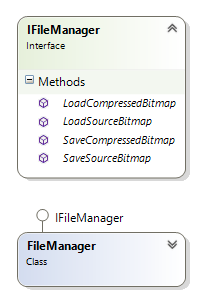
\includegraphics[scale=0.6]{IFileManager.png}
  \caption{ Интерфейс IFileManager }
  \label{fig:ifilemanager}
\end{figure}
IFileManager --- представляет интерфейс, который инкапсулирует работу с файловой системой(рисунок~\ref{fig:ifilemanager}).
Данный интерфейс был выделен для того, чтобы уменьшить зависимость алгоритма сжатия данных от способа хранения.
Следовательно, в будущем можно подобрать другие способы представления данных сжатых при помощи данного приложения.

В нем представлены методы:
\begin{itemize}
  \item LoadSourceBitmap() --- загрузка матрицы пикселей исходного изображения;
  \item SaveSourceBitmap() --- сохранение матрицы пикселей;
  \item LoadCompressedBitmap() --- загрузка матрицы пикселей из файла, содержащего сжатые данные нейронной сети;
  \item SaveCompressedBitmap() --- сохранение матрицы пикселей используя сжатие.
\end{itemize}

В прототипе представлена одна реализация FileManager, которая читает матрицы пикселей из файлов.
Также класс может FileManager сохранять и читать файлы с сжатыми изображниями.

\subsubsection{Интерфейс IImageComparer}
\label{subsub:development:types:iimagecomparer}

\begin{figure}[ht]
\centering
  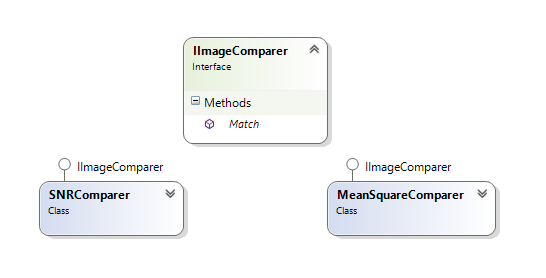
\includegraphics[scale=0.6]{IImageComparer.png}
  \caption{ Интерфейс IImageComparer }
  \label{fig:iimagecomparer}
\end{figure}
IImageComparer --- представляет интерфейс для сбора статистики по уровню искажений в полученных изображениях(рисунок~\ref{fig:iimagecomparer}).

В нем представлены методы:
\begin{itemize}
  \item Match() --- метод сравнивает исходное изображение и получившееся, вычисляя погрешность;
\end{itemize}

В прототипе представлены 2 реализации:
\begin{itemize}
  \item SNRComparer --- вычисляет отношение сигнал-шум;
  \item MeanSquareComparer --- вычисляет среднеквадратическое отклонение между изображениями.
\end{itemize}
